\documentclass{article}

\title{Homework 4}
\date{12-03-2023}
\author{Danny Zou}

\usepackage[left=.7in, right=.7in, top=0.5in, bottom=0.5in]{geometry}
\usepackage{amsmath}
\usepackage{indentfirst}
\usepackage{setspace}
\usepackage{graphicx}
\usepackage{multirow} 
\usepackage{amssymb}
\usepackage[table]{xcolor}


\newcommand{\boxedanswer}[1]{%

    \fbox{\large\textbf{#1}}%
}
\begin{document}
    \pagenumbering{gobble}
    \maketitle
    \onehalfspacing

    \section*{12.14.5}

    \noindent In the exercise, we examine in detail how an instruction is executed in singlecycle datapath. Problems in this exercise refer to a clock cycle in which the
processor fetches the following instruction word: 0xadac0014.

    \subsection*{(a) What are the values of the ALU control unit’s inputs
    for this instruction?}

    ALU control units inputs are:

    Opcode sw = \textbf{0010}

    ALUop = \textbf{00}

    \subsection*{(b) What is the new PC address after this instruction
    is executed? Highlight the path through which this
    value is determined.}

    \noindent The new PC address will be the current \boxed{\text{PC address} + 4} because each instruction is 4 bytes and PC always points to the next instruction.

    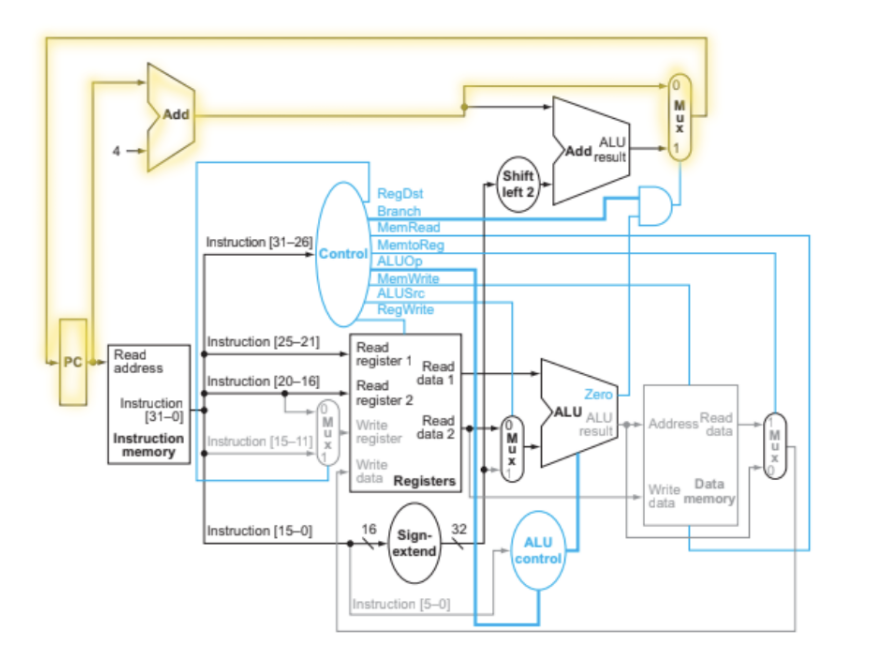
\includegraphics[width=0.8\linewidth]{highlight.png}

    Path Highlighted in yellow

    \newpage

    \subsection*{(c) For each mux, show the values of its inputs and outputs during the execution of this instruction. List
    values that are register outputs at Reg [xn]}

    There will be 3 muxes used.

    \subsubsection*{ALUSrc}
    
    Inputs : Reg[t4] and 0x0014

    Outputs : 0x0014

    \subsubsection*{MemToReg}
    
    Inputs : Reg[t5] + 0x0014 and Undefined Input

    Outputs : Undefined

    \subsubsection*{Branch}
    
    Inputs :  PC + 4 and PC + 0x28

    Outputs : PC + 4

    \subsection*{(d) What are the input values for the ALU and the two
    add units?}

    \subsubsection*{ALU}

    \$t5

    0x0014

    \subsubsection*{Two Add Units}

    PC + 4 Adder 

    \hspace{0.2in} -PC

    \hspace{0.2in} -4

    Branch Adder

    \hspace{0.2in} -PC

    \hspace{0.2in} -0x0028
    
    \subsection*{(e) What are the values of all inputs for the registers unit?}

    Read Register 1 = 0x13

    Read Register 2 = 0x12

    Write Register = Doesn’t Matter

    Write Data = Doesn’t Matter

    RegWrite = False

    \newpage

    \section*{12.14.7}

    \subsubsection*{(a) What is the latency of an R-type instruction(i.e., how
    long must the clock period be to ensure that this instruction works correctly)?}

    \noindent Latency of a R-Type Instruction = I-Mem/D-Mem + Register File + $(2 * Mux)$+ ALU + Register Read + Register
    Setup 

    \vspace*{0.1in}

    250ps + 150ps + $(2 * 25ps)$ + 200ps + 30ps + 20ps = \boxed{\textbf{700ps}}

    \subsubsection*{(b) What is the latency of lw? (Check your answer carefully. Many students place extra muxes on the critical
    path.)}

    \noindent Latency of Lw = Register Read + $(2 * I-Mem/D-Mem)$ + Register File + ALU + $(2 * Mux)$ + Register Setup

    \vspace*{0.1in}

    30ps + $(2 * 250ps)$ + 150ps + 200ps + $(2 * 25ps)$ + 20ps = \boxed{\textbf{950ps}}

    \subsubsection*{(c) What is the latency of sw? (Check your answer carefully. Many students place extra muxes on the critical
    path.)}

    \noindent Latency of Sw = Register Read + $(2 * I-Mem/D-Mem)$ + Register File + ALU + Mux

    \vspace*{0.1in}

    30ps + $(2 * 250ps)$ + 150ps + 200ps + 25ps = \boxed{\textbf{905ps}}

    \subsubsection*{(d) What is the latency of beq?}

    \noindent Latency of beq = Register Read + I-Mem/D-Mem + Register File + $(2 * Mux)$ + ALU + Single Gate + Register Setup

    \vspace*{0.1in}

    30ps + 250ps + 150ps + (2 * 25ps) + 200ps + 5ps + 20ps = \boxed{\textbf{705ps}}

    \subsubsection*{(e) What is the latency of an arithmetic, logical, or shift
    I-type (non-load) instruction?}

    \noindent Latency of I-type Instruction = Register Read + I-Mem/D-Mem + Register File + $(2 * Mux)$ + ALU + Register Setup

    \vspace*{0.1in}

    30ps + 250ps + 150ps + (2 * 25ps) + 200ps + 20ps = \boxed{\textbf{700ps}}

    \subsubsection*{(f) What is the minimum clock period for this CPU?}

    Mininum Clock Speed = \boxed{\textbf{950ps}}

    \newpage

    \section*{12.14.10}

    \subsection*{(a) What is the speedup achieved by adding this improvement?}

    Clock Cycle Time before improvements = 250 + 150 + 25 + 200 + 150 + 5 + 30 + 20 + 50 + 50 = 930ps

    Clock Cycle Time after improvements = 250 + 160 + 25 + 200 + 150 + 5 + 30 + 20 + 50 + 50 = 940ps

    $25 - (25 * 0.12) = 22$

    52 + 22 + 11 + 12 = 97 instructions after improvement

    Speed up = $\frac{\frac{930}{100}}{\frac{930}{97}} \approx 0.96$
    
    \subsection*{(b) Compare the change in performance to the change in
    cost.}

    Cost before improvements = 1000 + 200 + 10 + 100 + 30 + 2000 + 5 + 100 + 1 + 500 = 3946

    Cost per unit clock cycle before improvement = Cost / Clock cycle time = $\frac{3946}{930}$ = 4.24

    Cost after improvements = 1000 + 400 + 10 + 100 + 30 + 2000 + 5 + 100 + 1 + 500 = 4146

    Cost per unit clock cycle after improvement = Cost / Clock cycle time = $\frac{4146}{940}$ = 4.38

    Change in costs = 4.38 - 4.24 = 0.14

    Performance = 1/Latency

    Performance before improvements = $\frac{1}{100 * 930 * 10^{-12}} = 10.75 * 10^6$

    Performance after improvements = $\frac{1}{97 * 940 * 10^{-12}} = 10.967 * 10^6$

    Change in performance = $10.967 * 10^6 - 10.75 * 10^6 = 0.217 * 10^6$

    Cost Ratio = $\frac{4.38}{4.24} = 1.03$

    Performance Ratio = $\frac{10.967}{10.75} = 1.02$

    We see that the performance ratio is \textbf{1.02} while the cost ratio is \textbf{1.03}

    The Cost Ratio is higher than the Performance Ratio by \textbf{0.01}

    \subsection*{(c) Given the cost/performance ratios you just calculated, describe a situation where it makes sense to
    add more registers and describe a situation where it
    doesn’t make sense to add more registers.}

    \noindent If the priority is performace, adding more registers makes sense because adding more registers improve performance but increases cost. It streamlines instruction
    execution, enhancing overall system performance.

    \noindent Contrastly, if cost reduction is the priority, adding more registers may
    not be wise. Using fewer registers lowers costs but can compromise performance,
    as it increases the number of instructions and affects latency negatively.
    
    \noindent In summary, adding more registers is sensible when prioritizing performance,
    even with increased costs. However, if cost reduction is the main concern, adding
    more registers might not be the optimal choice due to potential performance
    trade-offs.
    
    \newpage

    \section*{12.14.16}

    \subsection*{(a) What is the clock cycle time in a pipelined and nonpipelined processor?}

    \subsubsection*{For a pipelined processor}

    Instructions Decode = 350ps

    Clock cycle time of pipelined processor = \boxed{\textbf{350ps}}

    \subsubsection*{For a non-pipelined processor}

    Clock cycle = IF + ID + EX + MEM + WB = 250ps + 350ps + 150ps + 300ps + 200ps = \boxed{\textbf{1250ps}}

    \subsection*{(b) What is the total latency of an lw instruction in a
    pipelined and non-pipelined processor?}

    \subsubsection*{For a pipelined processor}

    Total latency = \# of cycles * clock cycles = $5 * 350ps$ = \boxed{\textbf{1750ps}}

    \subsubsection*{For a non-pipelined processor}

    Total latency = IF + ID + EX + MEM + WB =  250ps + 350ps + 150ps + 300ps + 200ps = \boxed{\textbf{1250ps}} 

    \subsection*{(c)  If we can split one stage of the pipelined datapath
    into two new stages, each with half the latency of the
    original stage, which stage would you split and what
    is the new clock cycle time of the processor?}

    \noindent I would split the longest stage as it would be the best way to reduce the cycle
time. The new cycle time would then be calculated on the next longest stage.
Currently the longest stage is ID, so the new longest cycle time would be MEM
which is \boxed{\textbf{300ps}}

    \subsection*{(d)  Assuming there are no stalls or hazards, what is the
    utilization of the data memory?}

    Total utilization = Load instruction + store instruction

    Total utilization = 20\% + 15\%

    Total utilization = \boxed{\textbf{35\%}}

    \subsection*{(e) Assuming there are no stalls or hazards, what is the
    utilization of the write-register port of the ”Registers”
    unit?}

    Utilization of the write-register port = LW utilization + ALU utilization = 20\% + 45\% = \boxed{\textbf{65\% Clock Cycles}}



\end{document}